\documentclass{beamer}
\usepackage[latin1]{inputenc}
\usepackage{textpos}

\usepackage{graphics}
% \usepackage[demo]{graphicx}
\usepackage{adjustbox}

\usepackage[english]{babel}
\usepackage{colortbl}
\usepackage{caption}
% \usepackage{subcaption}
\usepackage{multirow}
\usepackage{amsmath}
\usepackage[makeroom]{cancel}
\usepackage{xcolor} % for colored text

\usepackage{tikz} % for flow charts
\usetikzlibrary{shapes,arrows,positioning,shadows,calc}

\usepackage{filecontents}% http://ctan.org/pkg/filecontents
\usepackage{silence}% http://ctan.org/pkg/silence
\WarningFilter{latex}{Overwriting file}% Remove LaTeX warnings starting with "Overwriting file"
\begin{filecontents*}{linereg.data}
#x y
0 4
10 24
\end{filecontents*} 

\begin{filecontents*}{linereg2.data}
#x y
2 8
8 20
\end{filecontents*} 

	\renewcommand<>{\item}[1]{\only#2{\beameroriginal{\item}{#1}}} % for replace a equation for other equation in the same place
	
	% \usetheme{Warsaw}
	\usetheme{Frankfurt}
	% \usetheme{Boadilla}
	\setbeamertemplate{navigation symbols}{} 
	% \useoutertheme{infolines} 
% \setbeamertemplate{footline}{\hbox{\vspace{0.1cm} \insertshortauthor \hspace*{3.5cm} \insertshorttitle \hspace*{4.0cm} \hfill\insertframenumber/\inserttotalframenumber}} 

\setbeamertemplate{footline}{\hbox{\vspace{0.1cm} \insertshortauthor \hspace*{3.5cm} \insertshorttitle \hspace*{4.4cm} \hfill\insertframenumber}} 

\def\braces#1{[#1]} % to define square parenthesis 
	
% \usecolortheme{orchid}

% \usecolortheme{lily}

% \usecolortheme{default}
\usecolortheme{cranejavier}

% \setbeamertemplate{footline}[frame number]
% \setbeamertemplate{footline}[page number]
	
	
	% -------------------------------------- Slide 1
	\title[Field Measurements and Instrumentation]{Intro to Instrumentation and Field Measurements in Remote Sensing}
	\author[J. Concha \& P. Romanczyk]{\Large Javier Concha and Paul Romanczyk}
	\institute{\footnotesize Digital Imaging and Remote Sensing Lab\\Chester F. Carlson Center for Imaging Science\\ Rochester Institute of Technology}
	\date{\today}


\AtBeginSection[ ]
{	\setbeamertemplate{footline}{} 	
	\begin{frame}{\LARGE Outline} 
	\LARGE
		\tableofcontents[currentsection]
	\end{frame}

\addtocounter{framenumber}{-1}	

\setbeamertemplate{footline}{\hbox{\vspace{0.1cm} \insertshortauthor \hspace*{2.0cm} \insertshorttitle \hspace*{3.8cm} \hfill\insertframenumber}} 
}	

% \AtBeginSubsection[ ]
% {		
% 	\begin{frame}{\LARGE Outline} 
% 		\tableofcontents[currentsection,currentsubsection]
% 	\end{frame}
% \addtocounter{framenumber}{-1}	
% }		
\newcounter{tmpc} % for resume counter
%&&&&&&&&&&&&&&&&&&&&&&&&&&&&&&&&&&&&&&&&&&&&&&&&&&&&&&&&&&&&&&&
%&&&&&&&&&&&&&&&&&&&&&&&&&&&&&&&&&&&&&&&&&&&&&&&&&&&&&&&&&&&&&&&
\begin{document}
{	
\setbeamertemplate{footline}{} 
\setbeamertemplate{headline}{}
	
	\begin{frame} 
	\titlepage
	
	\begin{textblock*}{10cm}(10.0cm,-8.2cm)
	   
\includegraphics[height=10mm]{/Users/javier/Desktop/Javier/MASTER_RIT/2011_THESIS/LaTeX/Presentation/tiger_walking_rit_color.eps}
	\end{textblock*}
	
	\begin{textblock*}{10cm}(-.7cm,-8.2cm)
	   
\includegraphics[height=10mm]{/Users/javier/Desktop/Javier/PHD_RIT/ConferencesAndApplications/2014_ASPRS_SOY/Images/dirs_logo.png}
	\end{textblock*}
	
	\begin{textblock*}{9cm}(2cm,-4.5cm)

	   \tikz\node[opacity=0.3]{ 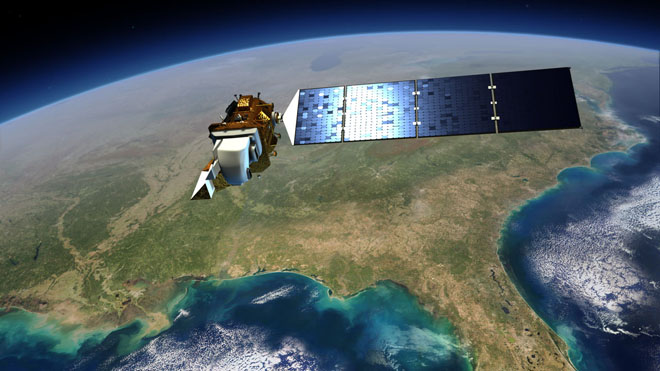
\includegraphics[width=65mm]{/Users/javier/Desktop/Javier/PHD_RIT/ConferencesAndApplications/2014_ASPRS_SOY/Images/landsat8-earth.jpg}};
	\end{textblock*}

	\begin{textblock*}{12cm}(3.0cm,0cm)
	   \scriptsize Presented for 2015 Intersession Term
	\end{textblock*}
	
	\end{frame}

}
\addtocounter{framenumber}{-1}
%\setbeamercovered{highly dynamic}
%\setbeamercovered{transparent}
\setbeamercovered{still covered={\opaqueness<1->{2}},again covered={\opaqueness<1->{2}}}

% ----------------------------------- Slide ----------------------------------------------	

\addtobeamertemplate{frametitle}{}{%
\begin{textblock*}{90mm}(8.2cm,-0.5cm)
% \includegraphics[height=0.5cm]{/Users/javier/Desktop/Javier/MASTER_RIT/SPIE2012/Slides/rit_white_no_bar.jpg}

\includegraphics[height=0.4cm]{/Users/javier/Desktop/Javier/PHD_RIT/ConferencesAndApplications/2014_ASPRS_SOY/Images/RIT_LOGO.png}
\end{textblock*}}


% ----------------------------------- Slide ----------------------------------------------
{
\setbeamertemplate{footline}{} 
\begin{frame}{\LARGE Outline} 
\LARGE
	\tableofcontents
\end{frame}

\addtocounter{framenumber}{-1}
}

%%%%%%%%%%%%%%%%%%% SECTION %%%%%%%%%%%%%%%%%%%%%%%%%%%%%%%%
\section{Introduction}
\subsection*{Motivation}
% --- slide ------------------------------------------------
\begin{frame}{\LARGE Course Goals} 
\LARGE
\begin{itemize}\itemsep.4cm
	\item Learn the importance of field measurements
	\item Learn how to take field measurements
	\item Learn about DIRS instruments
\end{itemize}
\end{frame}
% --- slide ------------------------------------------------
\begin{frame}{\LARGE Course Description} 
\LARGE
\begin{itemize}\itemsep.4cm
	\item Friday: Introduction
	\item Monday: Introduction (con't) and DIRS instruments exhibition
	\item Tuesday: Lab: Reflectance measurements
	\item Wednesday: Lab: LIDAR measurements
\end{itemize}
\end{frame}
% --- slide ------------------------------------------------
\begin{frame}{\LARGE Definitions} 
\LARGE
{\bf Field Measurements or Groundtruth:}\\
\vspace{.1cm}
``Observations or measurements made at or near the surface of the earth in support of remote sensing.''\\
\vspace{.5cm}
{\bf Remote Sensing:}\\
``Remote sensing is the science of obtaining information about objects or areas from a distance, typically from aircraft or satellites.''\\

\end{frame}
% --- slide ------------------------------------------------
\begin{frame}{\LARGE Motivation}
\LARGE
{\bf Why is it important?}\\
\begin{itemize}\itemsep.3cm
	\item Validation
	\item Calibration
	\item Correction
\end{itemize}
\end{frame}
% --- slide ------------------------------------------------
\begin{frame}{\LARGE Motivation}{\vspace{0.1cm} \Large Examples}
\vspace{-.7cm}
Include:\\
Javier's example (over water mea.)\\
Paul's example (LIDAR and trees?)

\end{frame}
% --- slide ------------------------------------------------
\begin{frame}{\LARGE Field Data Collection}{\vspace{0.1cm} \Large Area of Study}
\begin{figure}[htb]
  \centering
	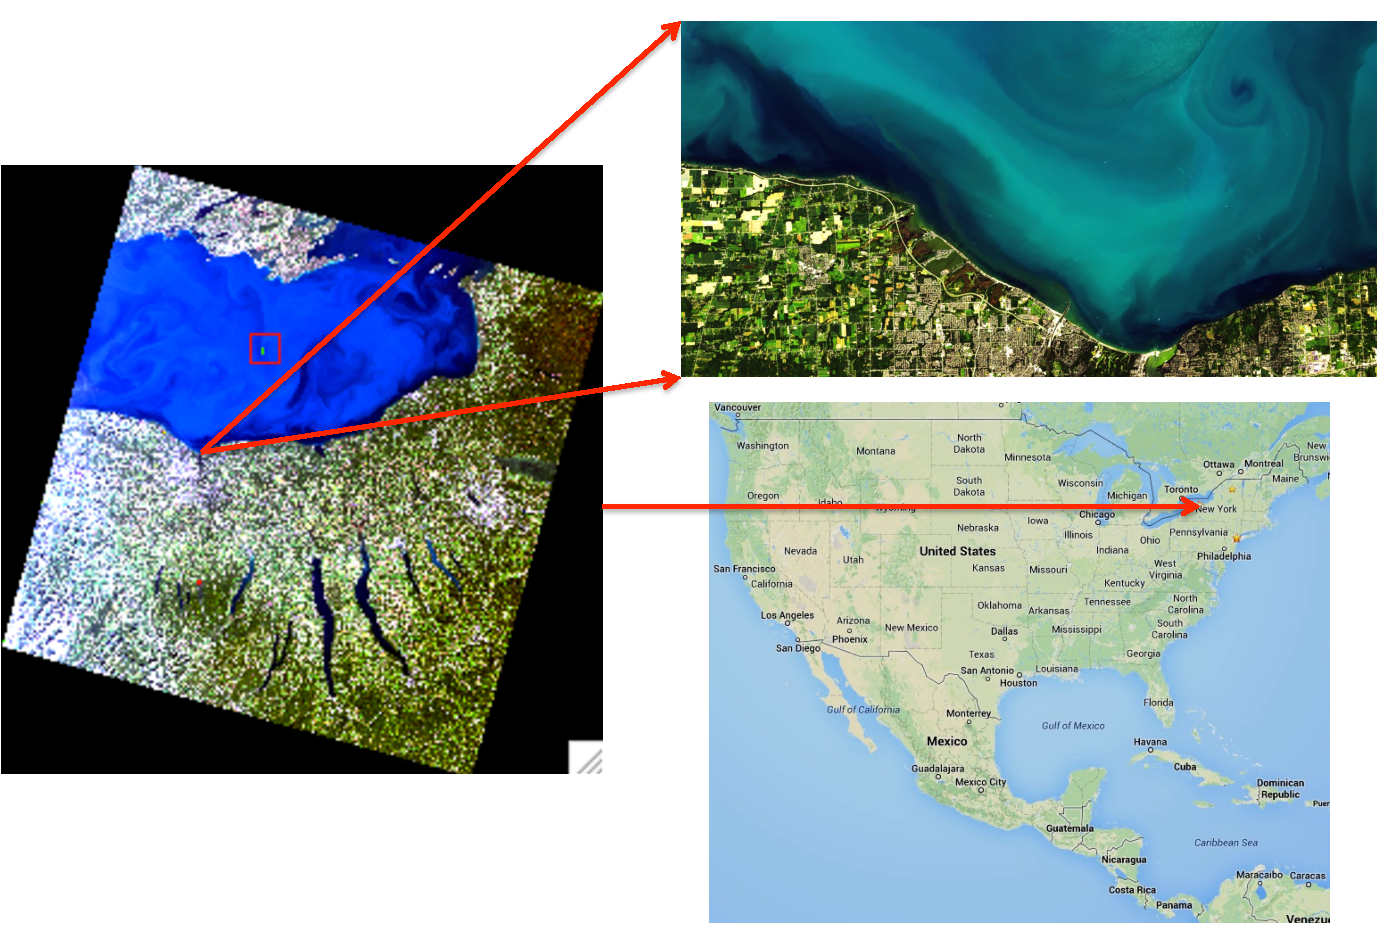
\includegraphics[height=7cm]{/Users/javier/Desktop/Javier/PHD_RIT/Latex/Proposal/Images/AreaOfStudy1.pdf} 
  % \caption{Sites in the Rochester Embayment for the water sample collection on September, $19^{th}$, 2013.\label{fig:0910913Sites} } 
\end{figure}
\end{frame}
% --- slide ------------------------------------------------
\begin{frame}{\LARGE Field Data Collection (con't)}{\vspace{0.1cm} \Large Area of Study}
\begin{figure}[htb]
  	\centering
  	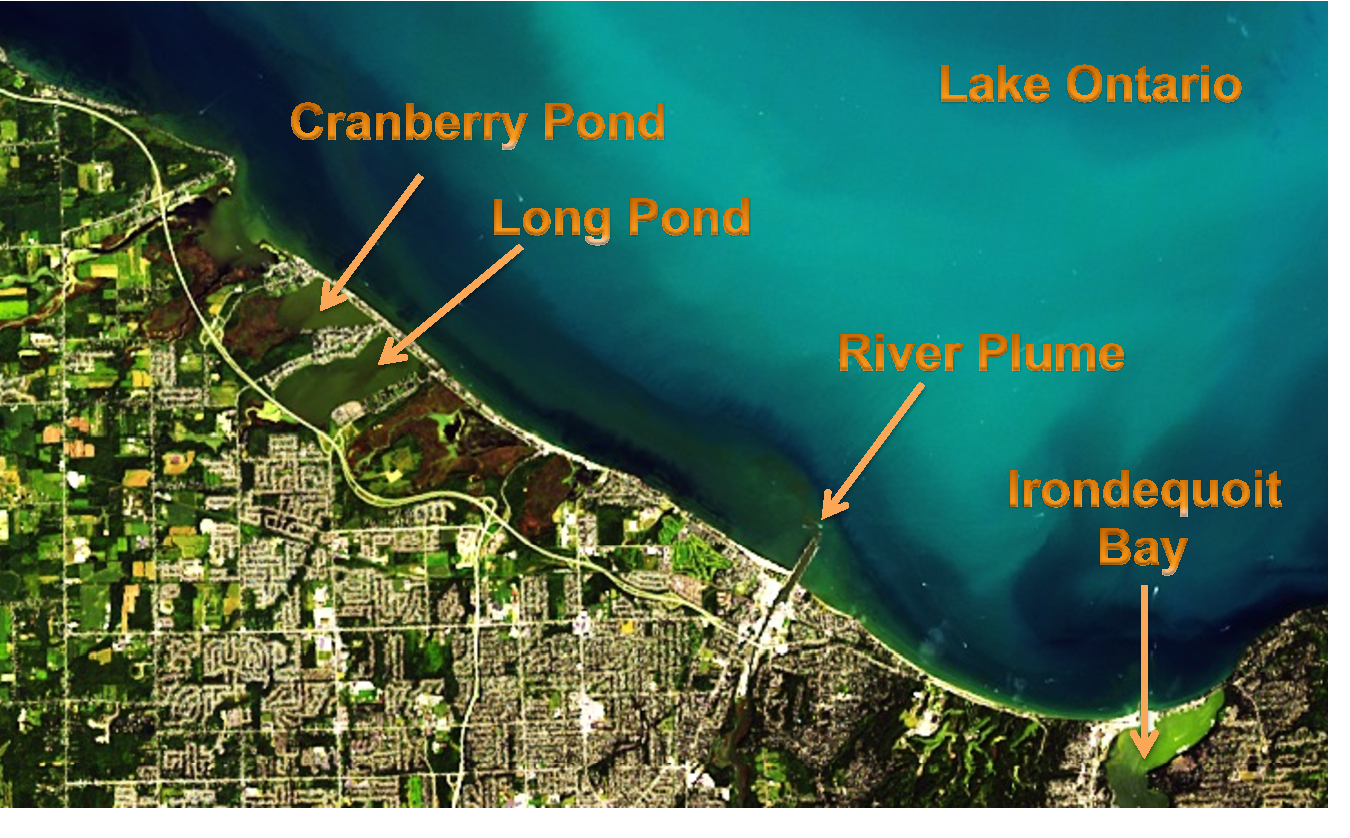
\includegraphics[height=6cm]{/Users/javier/Desktop/Javier/PHD_RIT/Latex/Proposal/Images/AreaOfStudy2.pdf}
\end{figure}
\end{frame}
% --- slide ------------------------------------------------
\begin{frame}{\LARGE Field Data Collection (con't)}
\vspace{-1cm}
\begin{figure}[htb]
\centering
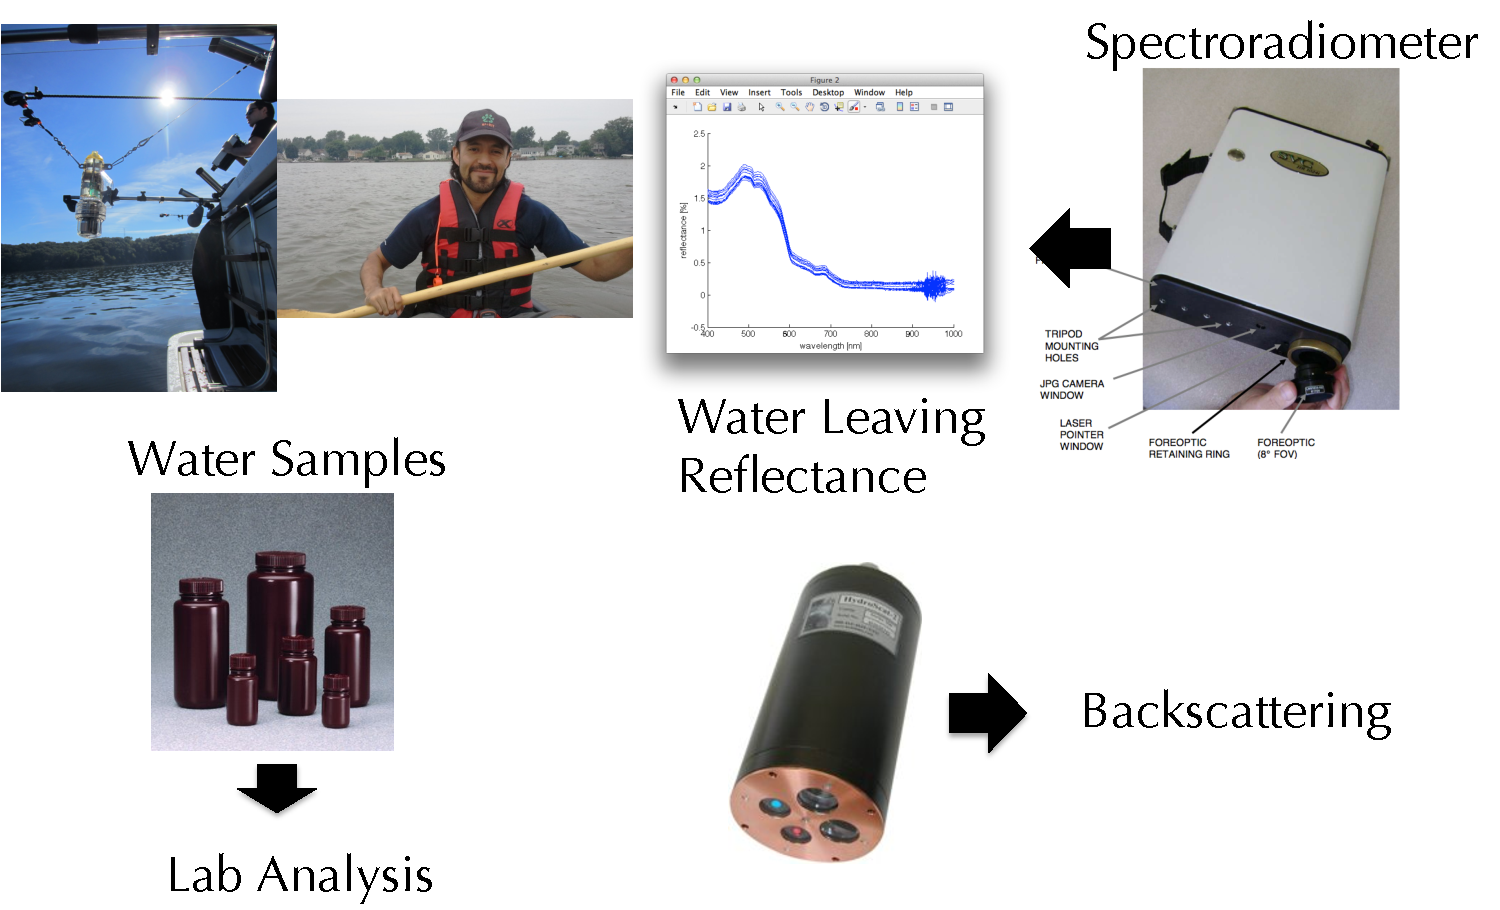
\includegraphics[height=7cm]{/Users/javier/Desktop/Javier/PHD_RIT/ConferencesAndApplications/2014_ASPRS_SOY/Images/Collection.pdf}
      
\end{figure}
% \centerline{Comparison between traditional ELM (dashed lines)}
% \centerline{and model-based ELM (solid lines).}
\end{frame}
% --- slide ------------------------------------------------
\begin{frame}{\LARGE Field Data Collection (con't)}{\Large Lab Measurements} 
\vspace{-1cm}
\begin{figure}[htb]
\centering
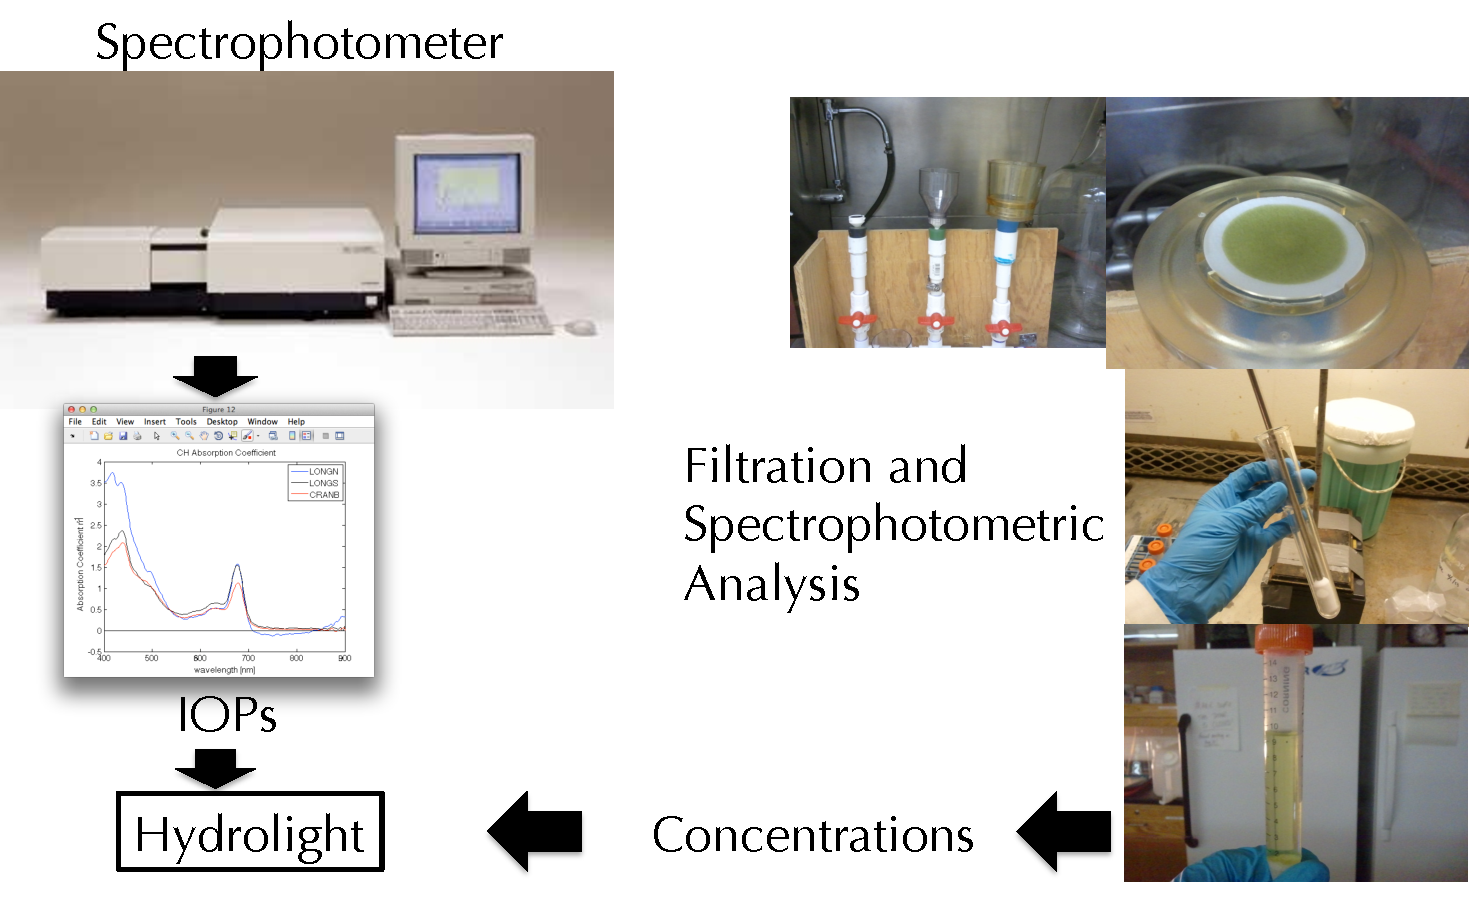
\includegraphics[height=7cm]{/Users/javier/Desktop/Javier/PHD_RIT/ConferencesAndApplications/2014_ASPRS_SOY/Images/LabMeasurements.pdf}
      
\end{figure}
% \centerline{Comparison between traditional ELM (dashed lines)}
% \centerline{and model-based ELM (solid lines).}
\end{frame}
% --- slide ------------------------------------------------
\begin{frame}{\LARGE Field Data Collection (con't)}{\vspace{0.1cm} \Large 2013 and 2014 Seasons}
\begin{table}[htb]
  
  \centering
  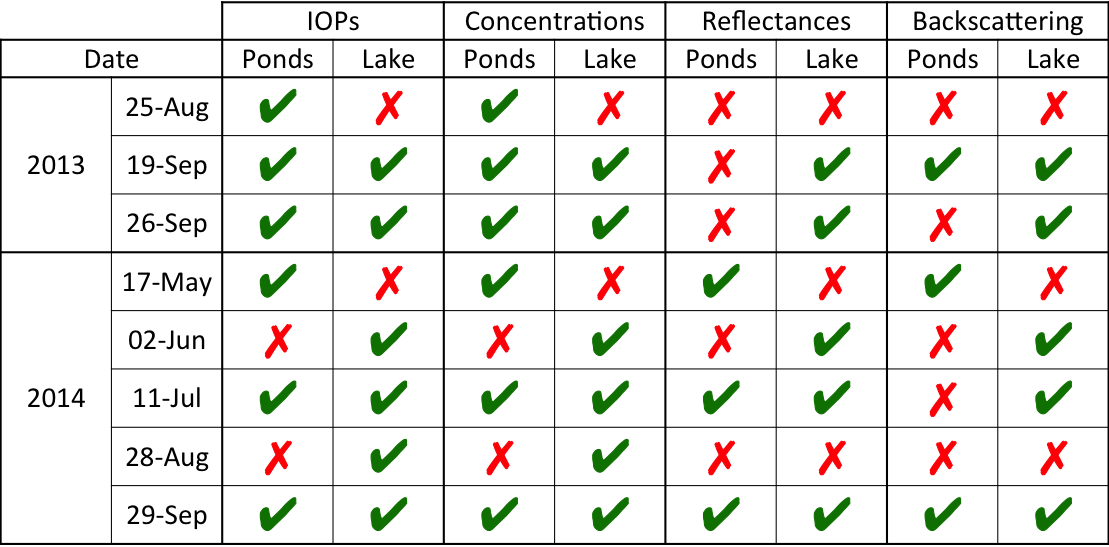
\includegraphics[width=11cm]{/Users/javier/Desktop/Javier/PHD_RIT/Latex/Proposal/Images/Collect1314.png}
  \label{tab:collect}
\end{table}
\end{frame}
%%%%%%%%%%%%%%%%%%% SECTION %%%%%%%%%%%%%%%%%%%%%%%%%%%%%%%%
\section{Background}
% --- slide ------------------------------------------------
\begin{frame}{\LARGE Kind of Measurements} 
\Large
\begin{itemize}\itemsep.4cm
	\item reflectance
	\item concentration
	\item location
\end{itemize}

\end{frame}
% --- slide ------------------------------------------------
\begin{frame}{\LARGE Radiometric Quantities: Radiance} 
% \begin{frame}{Radiometric Quantities: Radiance}
\begin{figure}[H]
\begin{columns}[t] % contents are top vertically aligned
	\begin{column}[T]{6cm} % each column can also be its own environment
  		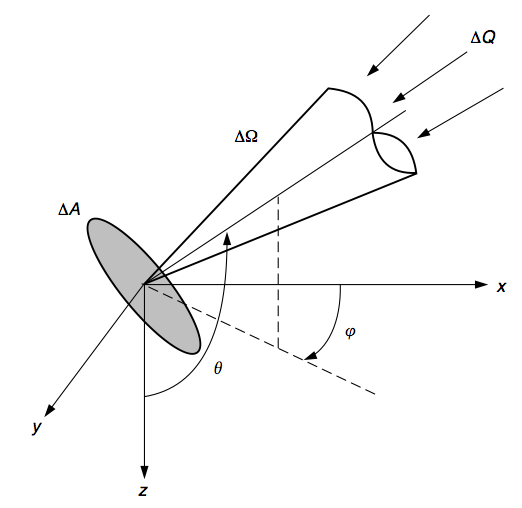
\includegraphics[height=6cm]{/Users/javier/Desktop/Javier/PHD_RIT/20123_Spring/Modeling/HydroLight/Beamer/RadianceDef.png}
    \end{column}
	\begin{column}[T]{4cm} % each column can also be its own environment
  		$\Delta Q$: radian energy incident \\
  		$\Delta t$: time interval \\
  		$\Delta A$: surface area at location (x,y,z)\\
  		$\Delta\Omega$: solid angle in direction ($\theta$,$\varphi$) \\
  		$\Delta\lambda$: photons wavelength interval
    \end{column}
\end{columns}	
\end{figure}
\only<1>{\begin{equation}
	\small L(x,y,z,t,\theta,\varphi,\lambda)\equiv\frac{\Delta Q}{\Delta t\Delta A\Delta\Omega\Delta\lambda}~~\left[ Js^{-1}m^{-2}sr^{-1}nm^{-1} \right]
		\end{equation}}
\only<2>{\begin{equation}
	\small L(x,y,z,t,\theta,\varphi,\lambda)\equiv\frac{\partial^4 Q}{\partial t\partial A\partial\Omega\partial\lambda}~~\left[ Js^{-1}m^{-2}sr^{-1}nm^{-1} \right]
		\end{equation}}
\end{frame}
% --- slide ------------------------------------------------
\begin{frame}{\LARGE Radiance Sensor} 
\begin{figure}
\centering
    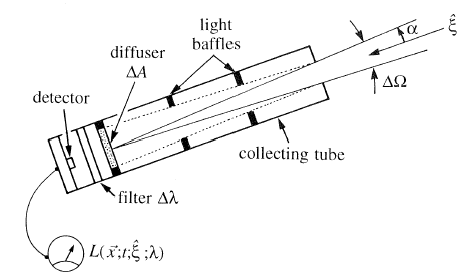
\includegraphics[height=5cm]{/Users/javier/Desktop/Javier/PHD_RIT/2014_Intersession/beamer/Images/RadianceSensor.png}
\end{figure}
\vspace{-.7cm}
\hfill \scriptsize (Source: \cite{MobleyOnline})

% \vspace{0.2cm}
% \centerline{Water Pixels}
% \centerline{(Unknown concentrations)}

\end{frame}
% --- slide ------------------------------------------------
\begin{frame}{Radiometric Quantities: Irradiance}
\textbf{Spectral downwelling scalar irradiance} at depth z:
\begin{equation}
	E_{od}(z,\lambda)=\int_{2\pi_d} L(z,\theta,\varphi,\lambda)d\Omega~~\left[Wm^{-2}nm^{-1} \right]
\end{equation}
\textbf{Spectral upwelling scalar irradiance} at depth z:
\begin{equation}
	E_{ou}(z,\lambda)=\int_{2\pi_u} L(z,\theta,\varphi,\lambda)d\Omega~~\left[Wm^{-2}nm^{-1} \right]
\end{equation}
\textbf{Spectral scalar irradiance} at depth z:
\begin{align}
	E_{o}(z,\lambda) &\equiv E_{od}(z,\lambda)+E_{ou}(z,\lambda)\\
					 &=\int_{4\pi} L(z,\theta,\varphi,\lambda)d\Omega
\end{align}
\end{frame}
% --- slide ------------------------------------------------
\begin{frame}{\LARGE Scalar Irradiance Sensor} 
\begin{figure}
\centering
    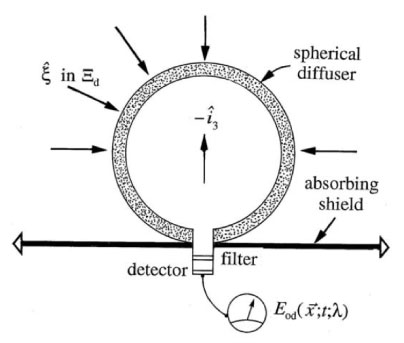
\includegraphics[height=5cm]{/Users/javier/Desktop/Javier/PHD_RIT/2014_Intersession/beamer/Images/ScalarIrradianceSensor.jpg}
\end{figure}
\vspace{-.7cm}
\hfill \scriptsize (Source: \cite{MobleyOnline})

% \vspace{0.2cm}
% \centerline{Water Pixels}
% \centerline{(Unknown concentrations)}

\end{frame}
% --- slide ------------------------------------------------
\begin{frame}{Radiometric Quantities: Irradiance}
\textbf{Spectral downwelling plane irradiance} at depth z:
\begin{equation}
	E_{d}(z,\lambda)=\int_{2\pi_d} L(z,\theta,\varphi,\lambda)|cos\theta|d\Omega~~\left[Wm^{-2}nm^{-1} \right]
\end{equation}
Photosynthetic available radiation, \textbf{PAR}:
\begin{equation}
	PAR(z)\equiv \int_{350nm}^{700nm} \frac{\lambda}{hc}E_o(z,\lambda)d\lambda~~~\left[photons~s^{-1}m^{-2} \right]
\end{equation}
\end{frame}
% --- slide ------------------------------------------------
\begin{frame}{\LARGE Planar Irradiance Sensor} 
\begin{figure}
\centering
    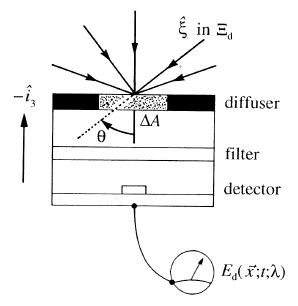
\includegraphics[height=5cm]{/Users/javier/Desktop/Javier/PHD_RIT/2014_Intersession/beamer/Images/PlaneIrradianceSensor.png}
\end{figure}
\vspace{-.7cm}
\hfill \scriptsize (Source: \cite{MobleyOnline})

% \vspace{0.2cm}
% \centerline{Water Pixels}
% \centerline{(Unknown concentrations)}

\end{frame}
% --- slide ------------------------------------------------
\subsection*{}
\begin{frame}{Reflectance}
\begin{itemize}\itemsep.4cm
	\item {\textbf{Irradiance reflectance:}\\
			\begin{equation}
				R(z,\lambda)\equiv \frac{E_u(z,\lambda)}{E_d(z,\lambda)}
			\end{equation}}\\
	\item{ \textbf{Remote sensing reflectance (water):}\\
			\begin{equation}
				R_{rs}(\theta,\varphi,\lambda)\equiv \frac{L_w(\theta,\varphi,\lambda)}{E_d(\lambda)}~~\left[sr^{-1} \right]
			\end{equation}\\
			where $L_w$ is the \textbf{water-leaving radiance}\\}
	\item{ \textbf{Bidirectional Reflectance Distribution Function (BRDF):}\\
			\begin{equation}
				r_{BRDF} = \frac{\displaystyle L(\theta_o,\phi_o)}{\displaystyle E(\theta_i,\phi_i)}~~~\left[sr^{-1}\right]
			\end{equation}}
\end{itemize}
\end{frame}
%%%%%%%%%%%%%%%%%%% SECTION %%%%%%%%%%%%%%%%%%%%%%%%%%%%%%%%
\section{Taking Measurements}
% --- slide ------------------------------------------------
\begin{frame}{\LARGE Remote-Sensing Reflectance}
 	\begin{columns}[c] % contents are top vertically aligned
  		\begin{column}[T]{5cm} % each column can also be its own environment
  		\begin{itemize}
  		\item 3 measurements:
	  		\begin{itemize}
	  			\item {$L_g$ (spectralon)}
	  			\item {$L_t = L_r+L_w$ (water)}
	  			\item {$L_{sky}$}
	  		\end{itemize}
	  	\item{Remote-sensing reflectance:\\
	  			\vspace{-0.5cm}
	  			\begin{gather*} 
	  				R_{rs} = L_w/E_d\\
	  				= (L_t - L_r)/E_d
	  			\end{gather*}\\
	  			with $L_r = 0.028*L_{sky}$}	
	  	
	  	\item {$E_d = L_g*\pi$}
	  	\item {$\phi:$ azimuthal angle}
	  	\item {$\theta:$ zenith angle}
  		\end{itemize}
    	\end{column}
    	\hspace{-1cm}
    	\begin{column}[T]{7cm} % each column can also be its own environment
  			\begin{figure}[htb]
				\centering
				 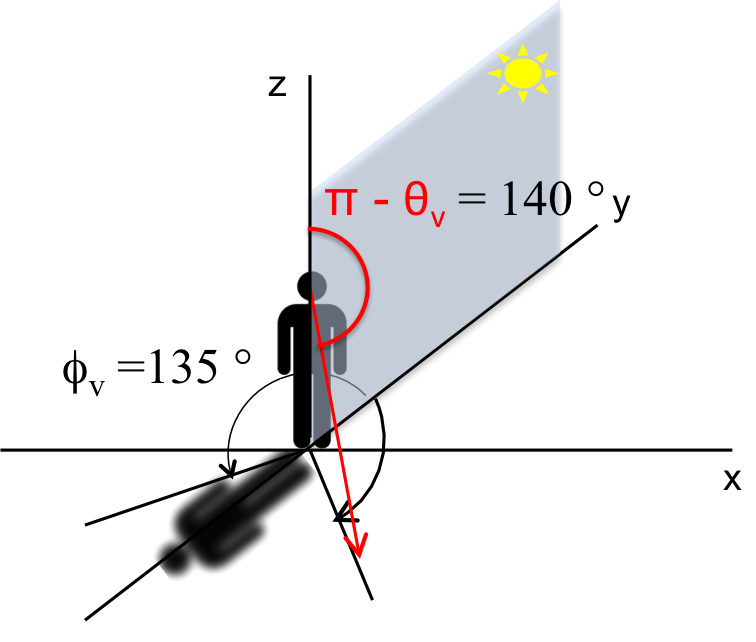
\includegraphics[height=6cm]{/Users/javier/Desktop/Javier/PHD_RIT/2014_Intersession/beamer/Images/LwGeometry.png}
			\end{figure}
 
    	\end{column}
    \end{columns}
\end{frame}

% --- slide ------------------------------------------------
\begin{frame}{$L_{sky}$}

\begin{figure}[htb]
				\centering
				 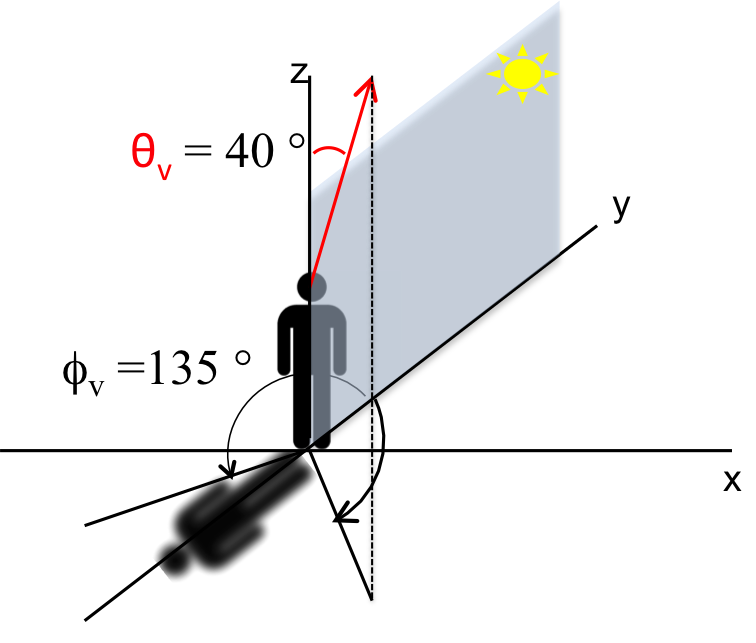
\includegraphics[height=6cm]{/Users/javier/Desktop/Javier/PHD_RIT/2014_Intersession/beamer/Images/LskyGeometry.png}
			\end{figure}

\end{frame}
% --- slide ------------------------------------------------
\begin{frame}{Diffuse white reference panel (Spectralon)}
\begin{columns}[c] % contents are top vertically aligned
  	\begin{column}[T]{5cm}

		\begin{itemize}\itemsep.4cm
			\item{For a Lambertian surface:\\
				\vspace{.1cm}
				$L = \frac{\displaystyle E_dr}{\displaystyle \pi} \Rightarrow E_d = \frac{\displaystyle  L\pi}{\displaystyle r}$}
			\item{ For spectralon $r\approx 1$ ($\approx 100\%$)\\
			$\Rightarrow E_d = L\pi$}
		\end{itemize}
	\end{column}	
	\begin{column}[T]{7cm} % each column can also be its own environment
	  			\begin{figure}[htb]
					\centering
					 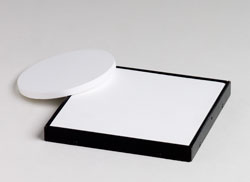
\includegraphics[height=3cm]{/Users/javier/Desktop/Javier/PHD_RIT/2014_Intersession/beamer/Images/spectralon-web.jpg}
				\end{figure}
				\begin{figure}[htb]
					\centering
					 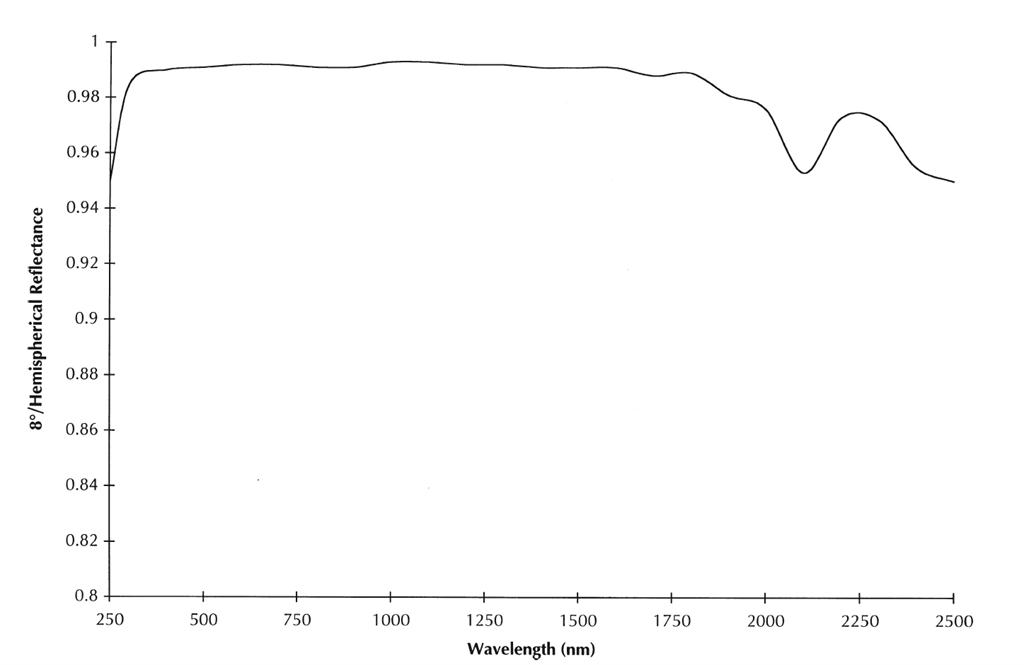
\includegraphics[height=3cm]{/Users/javier/Desktop/Javier/PHD_RIT/2014_Intersession/beamer/Images/SpectralonTargetsReflectance.jpg}
				\end{figure}
	 
	\end{column}
\end{columns}
\end{frame}
%%%%%%%%%%%%%%%%%%% SECTION %%%%%%%%%%%%%%%%%%%%%%%%%%%%%%%%
% \section{Conclusions}
% \subsection*{Conclusions}
% % --- slide ------------------------------------------------
% \begin{frame}{\LARGE Conclusions}

% \Large
% \begin{itemize}\itemsep.4cm
% 	\item Current retrieval algorithm depends on IOPs from the field. Not always available!

% 	\item LUT from Hydrolight: Highly dependent in phase function

% 	\item Obtain field data for Landsat-8 is difficult, mainly for weather conditions
% \end{itemize}

% \end{frame}

% --- slide ------------------------------------------------
{	
\setbeamertemplate{footline}{} 
\setbeamertemplate{headline}{}
\begin{frame}[noframenumbering] 

\vspace{\baselineskip}
\centerline{\Large Thanks for your attention!}
	\vspace{\baselineskip}
\vspace{-.3cm}
% \centerline{\Huge QUESTIONS?}
\uncover <2->{\centerline{\Huge QUESTIONS?}}
\vspace{\baselineskip}
\centerline{Javier A. Concha}
\centerline{jxc4005@rit.edu}

\begin{figure}[htb]
\centering
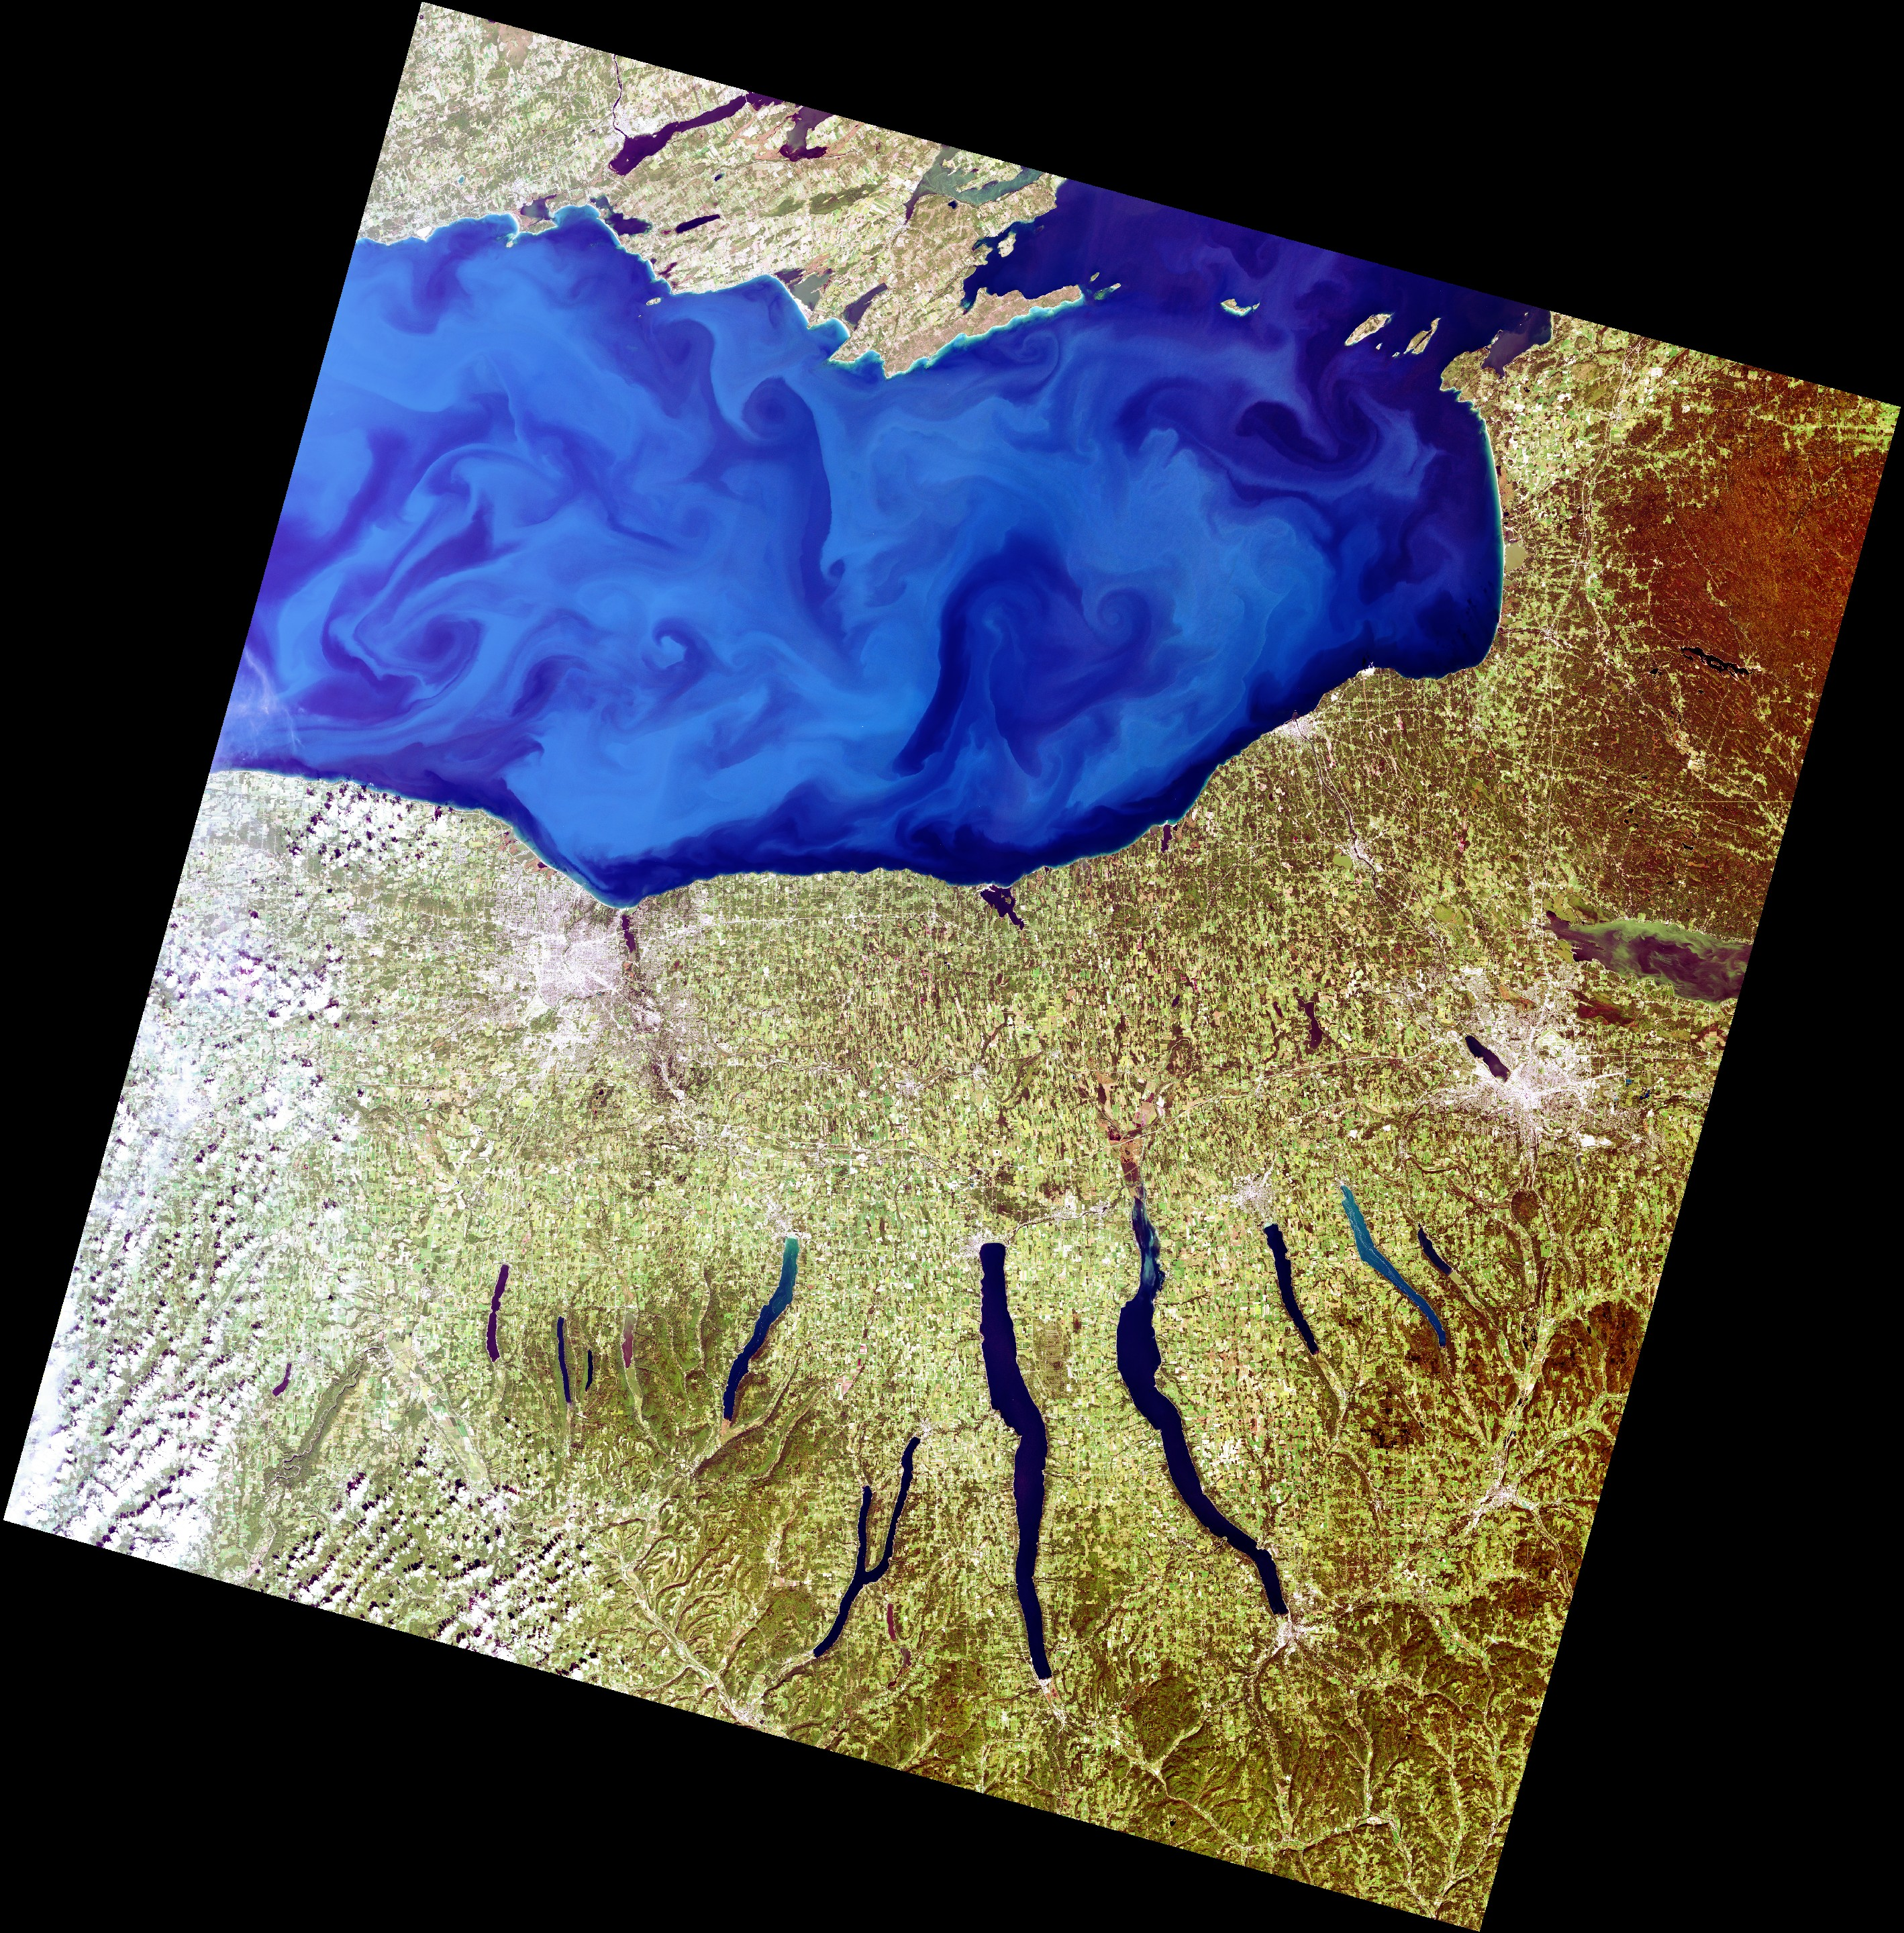
\includegraphics[height=5cm]{/Users/javier/Desktop/Javier/PHD_RIT/ConferencesAndApplications/2014_ASPRS_SOY/Images/LC80160302013262LGN00.jpg}
\end{figure}
\vspace{-.5cm}
\centerline{\tiny (09/19/2013)}
\end{frame}
}
% % BIBLIOGRAPHY
% \bibliographystyle{apalike}

% \bibliography{/Users/javier/Desktop/Javier/PHD_RIT/Latex/javier_bib}
% --- slide ------------------------------------------------
\section*{}
\begin{frame}%[shrink=30] 
\tiny
  \frametitle{References}
  % \nocite{*}
  \bibliographystyle{apalike}
  \bibliography{/Users/javier/Desktop/Javier/PHD_RIT/Latex/javier_bib}
\end{frame}
\end{document} 
% EEEEEEEEEEENNNNNNNNNNNNNNDDDDDDDDDDDD